\documentclass[11pt]{article}

\usepackage{latexsym}
\usepackage{amsmath}
\usepackage{amssymb}
\usepackage{amsthm}
\usepackage{graphicx}
\usepackage{listings}
\graphicspath{ {./images/} }
\usepackage{wrapfig}
% \usepackage{pseudocode}
\usepackage{url}

\usepackage[backref, colorlinks=true, citecolor=red, urlcolor=blue, pdfauthor={Prakash Dhimal}]{hyperref}
\usepackage{chngcntr}
% does not reset figure counter.
\counterwithout{figure}{section}

% 1-inch margins, from fullpage.sty by H.Partl, Version 2, Dec. 15, 1988.
\topmargin 0pt
\advance \topmargin by -\headheight
\advance \topmargin by -\headsep
\textheight 8.9in
\oddsidemargin 0pt
\evensidemargin \oddsidemargin
\marginparwidth 0.5in
\textwidth 6.5in

% %%%%%%%%%%%%%%%%%%%%%%%%%%%%%%%%%%%%%%%%%%%%%%%%%%%%%%%%%%
% SET THE TITLE
% %%%%%%%%%%%%%%%%%%%%%%%%%%%%%%%%%%%%%%%%%%%%%%%%%%%%%%%%%%

% TITLE:
\title{Predicting the Impact of COVID-19
}

% AUTHORS:
\author{William Austin\\% Name author
    \href{mailto:waustin3@gmu.edu}{\texttt{waustin3@gmu.edu}} %% Email author 1 
\and Prakash Dhimal\\% Name author
    \href{mailto:pdhimal@gmu.edu}{\texttt{pdhimal@gmu.edu}} %% Email author 2
    }
    
% DATE:
\date{\today}

\parindent 0in
\parskip 1.5ex
%\renewcommand{\baselinestretch}{1.25}

\begin{document}
\maketitle
\begin{abstract}

The coronavirus (COVID-19) outbreak caused by the 2019 Novel Coronavirus (2019-nCov) has become a global pandemic, with more than 4 million people infected, and hundreds of thousands of deaths around the globe. Countries across the globe are taking action to control the spread, but there is significant uncertainty about what the future holds. Predicting when the spread of the virus will peak using compartmental modeling in epidemiology has been a huge focus among government, academic institutions, and the private sector. In this paper, we discuss the basic compartmental model in epidemiology, the SIR model, and use data mining techniques to fit the SIR model curve with COVID-19 data. Our goal is to forecast the spread of COVID-19 confirmed cases, fatalities, and recoveries in different countries around the world.

\subsection{Summary of the report}

The structure of this paper is as follows. In section 1, we introduce COVID-19 and the basic compartmental model in epidemiology, the SIR model. In Section 2 we briefly discuss related work. In section 3, we present the solution to our problem. In Section 4.1, we discuss the data that we used for this project. Section 4.2 dives into the set-up of the SIR model. In section 5, we discuss our results and give our analysis on those results. In section 6, we discuss the evaluation metrics used to evaluate the performance of our model. Section 7, concludes the paper.
\end{abstract}

\section{Introduction}

The coronavirus (COVID-19) outbreak, also known as COVID-19 was first reported by Wuhan Municipal Health Commission, China on 31st December 2019 and has since spread to the vast majority of countries. The World Health Organization (WHO) declared COVID-19 as a Public Health Emergency of International Concern (PHEIC) on January, 30th 2020 \cite{who-website}. Since then, the outbreak has become a global pandemic, with more than 4 million people infected, and hundreds of thousands of deaths around the globe. COVID-19 is not only causing mortality but is also putting considerable stress on the health systems of countries across the globe. Countries across the globe are taking action to control the spread, but there is significant uncertainty about what the future holds. As shown in figure \ref{fig:covid-cases-daily-changes-us}, COVID-19 cases in the United States have been hovering around all-time highs, while the country and specific states are getting ready loosen social distancing measures put in place to control the spread of the disease. This project's goal is to use the principles of data mining and mathematical models of epidemic spread to forecast the spread of COVID-19 cases, deaths, and recoveries. This paper aims to deliver an overview of the SIR model and the outcome of our simulation by using the dataset of COVID-19.

\begin{figure}[h]
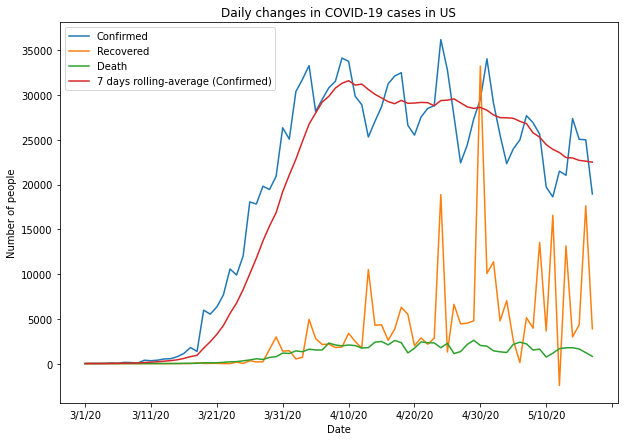
\includegraphics[width=14cm, height=9cm]{images/daily-numbers.png}
\centering
\caption{Daily changes in COVID-19 cases in the US (03/01/2020 - 05/17/2020)}
\label{fig:covid-cases-daily-changes-us}
\end{figure}

% reference example
% Figure \ref{simple-point-cloud} shows

\section{Related work}
In recent weeks, academic institutions, government, and industry researchers have put in a lot of effort into using Artificial Intelligence, Machine learning, and Data mining techniques to model the spread of the Novel Coronavirus. There is a large body of research and data around Covid-19 posted on Kaggle and other platforms to help scientists collaborate on this problem at unprecedented levels. Governments and organizations involved in COVID-19 response across the globe are adopting data mining techniques to assist in analyzing the spread of the virus.

The Institute for Health Metrics and Evaluation (IHME) \cite{ihme}, developed a curve-fitting model that looks at how the disease progressed in other geographies, like China, Italy, and Spain, and tries to extrapolate a prediction from there. IHME’s model mainly uses statistical model estimation for population death rate and health service utilization. 

An excellent introduction to the most prominent models being currently developed for projections in the US is given by FiveThirtyEight \cite{latest-models}. Current projections and a discussion of the models from IMHE, MIT, University of Massachusetts, Columbia University, University of Texas, and others are included. While most organizations are utilizing a compartmental model to generate predictions, there are major differences in the design of the models, parameters, and data sets being incorporated. A few of the highlights are:
\begin{itemize}
    \item The University of Texas model makes an effort to incorporate the effect of social distancing and uses different assumptions than IMHE to fit the model to the data. Social distancing metrics based on information reported by mobile devices are used.
    \item The MIT model is based on an SEIR model and tries to quantify the effects of government interventions.
    \item The University of Massachusetts model is based on a Bayesian compartmental model and makes predictions based on the prior distribution of the data.
    \item The Columbia University model is based on county-level data from across the US and hospital bed counts. Its projections are focused on generating several future scenarios at varying confidence levels.
\end{itemize}

As we see, the vast majority of the COVID-19 scenarios and forecasts have been based on mathematical compartmental models that capture the probability of moving between Susceptible, Infected, and Recovered (SIR) states. While any model is only as good as the assumptions we make, these models, in particular, are sensitive to assumptions and the results differ considerably. In our work, we use a curve-fitting model to uncover the parameters that are used in this model and have used official sources like the WHO and the CDC to make assumptions where needed. We call this the \textbf{curve fitted SIR model}. Later in this report, we will give an overview of compartmental models and in particular, we will show the equations and intuition describing the behavior of the SIR model.

\section{Solution}

Our analysis of this problem begins by looking at the existing work done in this area, as described in the previous section. Additionally, we considered the data sources that were available to us for experimentation. The Johns Hopkins University COVID-19 Data Repository contains daily values for confirmed cases, recovered individuals, and deaths, broken down by country and region. With access to this data, we were able to plot it and see how the data resembles the output of a Suspected-Infected-Removed (\textbf{SIR}) model in many cases. We describe additional details about the data set later in this report.

The SIR model is one of the simpler approaches to looking at the spread of infectious diseases, so it became a very useful starting point for us. One of the main reasons for this simplicity is that there are only two parameters ($\beta$ and $\gamma$) for the model, describing the rate of flow of individuals between the three states. This was advantageous for us because we can determine exact historical values for these parameters, based on the data set.

Our next activity was to graph the historical values for $\beta$ and $\gamma$. After doing this, it became obvious that the true values will vary over time. However, this makes sense, because the actual values of these parameters are a reflection of what happens in the world, which is a result of human behavior, and can change over time. An example graph of the changes in the value of beta across the historical data range is shown below.

\begin{figure}[h]
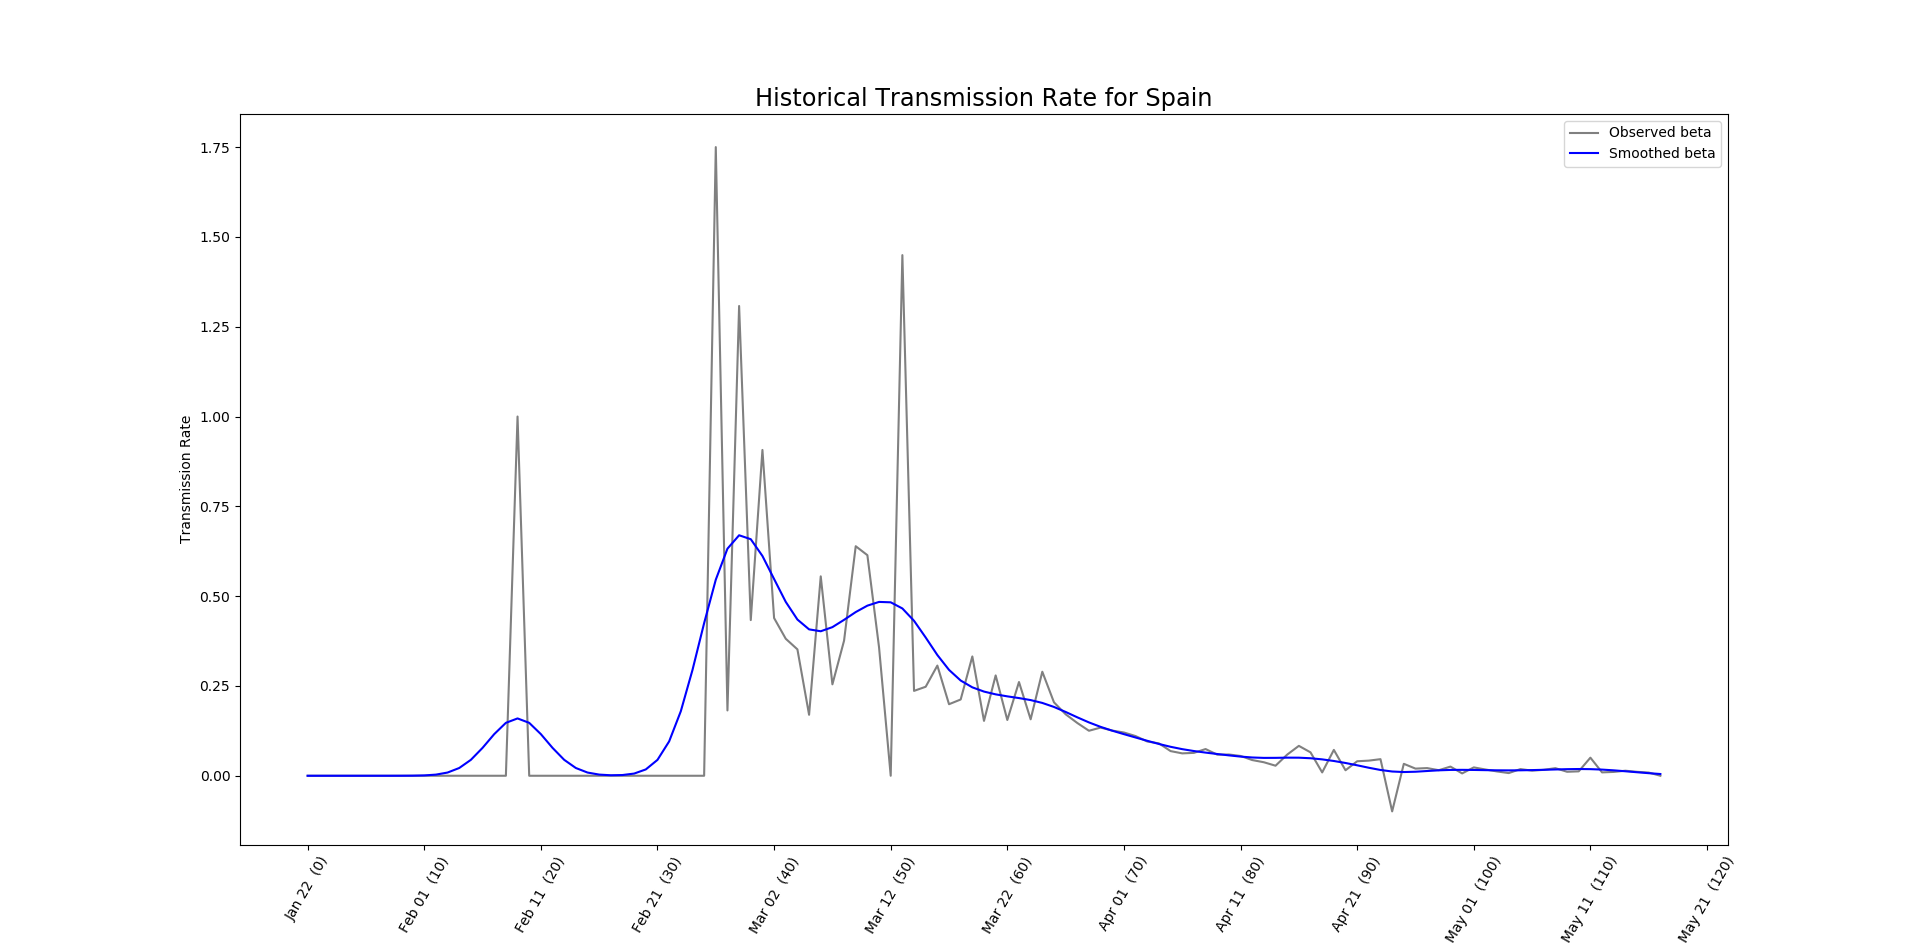
\includegraphics[width=15cm]{images/SampleBetaChart.png}
\centering
\caption{Historical Beta Values for Spain, with Smoothing}
\label{fig:sample-beta}
\end{figure}

Based on these results, the remainder of our project work was aimed at generating predictions for what the future could look like by estimating the value of $\beta$ and $\gamma$ and applying the SIR model equations. Although these equations can be applied to any future time, the SIR model is extremely sensitive to these parameters, so we typically only generate 30 days of predictions.

By focusing on estimating the parameter values for the SIR model, we can try to attack it as a regression problem. In our case, we imagine that the true value of $\beta$ on day $t$ can be given by the function $\beta(t)$. Likewise, we can also imagine that the true value of $\gamma$ is represented by $\gamma(t)$ on day $t$. However, as the graph above shows, these functions do not fall into a clear category. Therefore, we tried several extrapolation techniques. This includes:

\begin{itemize}
    \item Linear Regression
    \item Quadratic Regression
    \item Weighted Average of $\beta(t)$ values with Exponential Decay
    \item Weighted Average of $\beta'(t)$ values (Slope) with Exponential Decay
    \item Neural Network Regression
\end{itemize}

With this set of models, our next step was to incorporate the historical data to validate how accurate the predictions are for a given prediction range. We can then compare the errors for all candidate models, choose the one with the lowest error, and use it to make predictions for future time frames. More information about the details of this process is included in the rest of the report.

\section{Experiments}
\subsection{Data}
We use the Novel Coronavirus COVID-19 Data Repository from Johns Hopkins University’s Center for Systems Science and Engineering (CSSE) \cite{JHU-data} as our main data source. This data set provides total counts of how many cases have been confirmed, broken down by country and region/province. This is a time-series data and the number of cases on any given day is the cumulative number. These time-series data are for global confirmed cases, recovered cases, and deaths. Australia, Canada, and China are reported at the province/state level. The US and other countries are at the country level. In addition, it is an aggregated data source, so it is based on contributions from organizations around the world, including the WHO (World Health Organization) and various other public organizations around the world.

This data is updated every day since COVID-19 cases are evolving daily in different parts of the world. We have collected the data up to the date of this report. Therefore, we are using partial data sets. However, we were able to build and test models based on data collected up to this point.

After acquiring the data from the data source, we represented the data as a matrix (table). We aggregated the data on the country level. We then removed the features that we didn't need for this analysis and created features that we needed. We implemented stratified sampling to split the time series data collected so far into the training set and testing set.

In addition to the daily data provided by JHU, for accurate predictions, we also need to know what the current population of each country or region in the data set is. To get these figures, we downloaded a simple data set from Kaggle \cite{population-csv} and modified it slightly so that the country labels match between the two data sources.

For each country, before any COVID-19 cases have been reported, all individuals are considered susceptible, so this population value is used in our calculations for the initial condition, $S(0)$. In addition, we also sometimes choose to scale the $\beta$ variable by the population count to give a more literal interpretation of the constant.

\subsection{Modeling infectious disease}
\subsubsection{SIR model}
One of the best ways to model infectious diseases like COVID-19 is to use a compartmental model. A compartmental model separates the population into several compartments. The \textbf{SIR} model is one of the compartmental models used for modeling epidemics. In this model we divide the population (of a country, state, city, etc) into three groups:
\begin{enumerate}
    \item \textbf{S}usceptible: This is a group of individuals that have not been infected with the disease at time (t). This means that this group of people are susceptible to the disease.
    \item\textbf{I}nfectious: This group of individuals are currently infected with the disease at time (t) and are capable of spreading the disease to those in the susceptible category. Those Infected are expected to recover at a certain time in the future and gain “immunity”.
    \item \textbf{R}emoved: This group of individuals have already caught the virus, and cannot be infected again (Recovered), or unfortunately lost their lives (Dead). Here we assume that once you get the virus and recover from it, you gain some sort of immunity against the virus. In most SIR modeling, this group is referred to as Recovered. Since we are combining the Recovered and Death into the same group, we decided to call it Removed. 
\end{enumerate}

\begin{figure}[h]
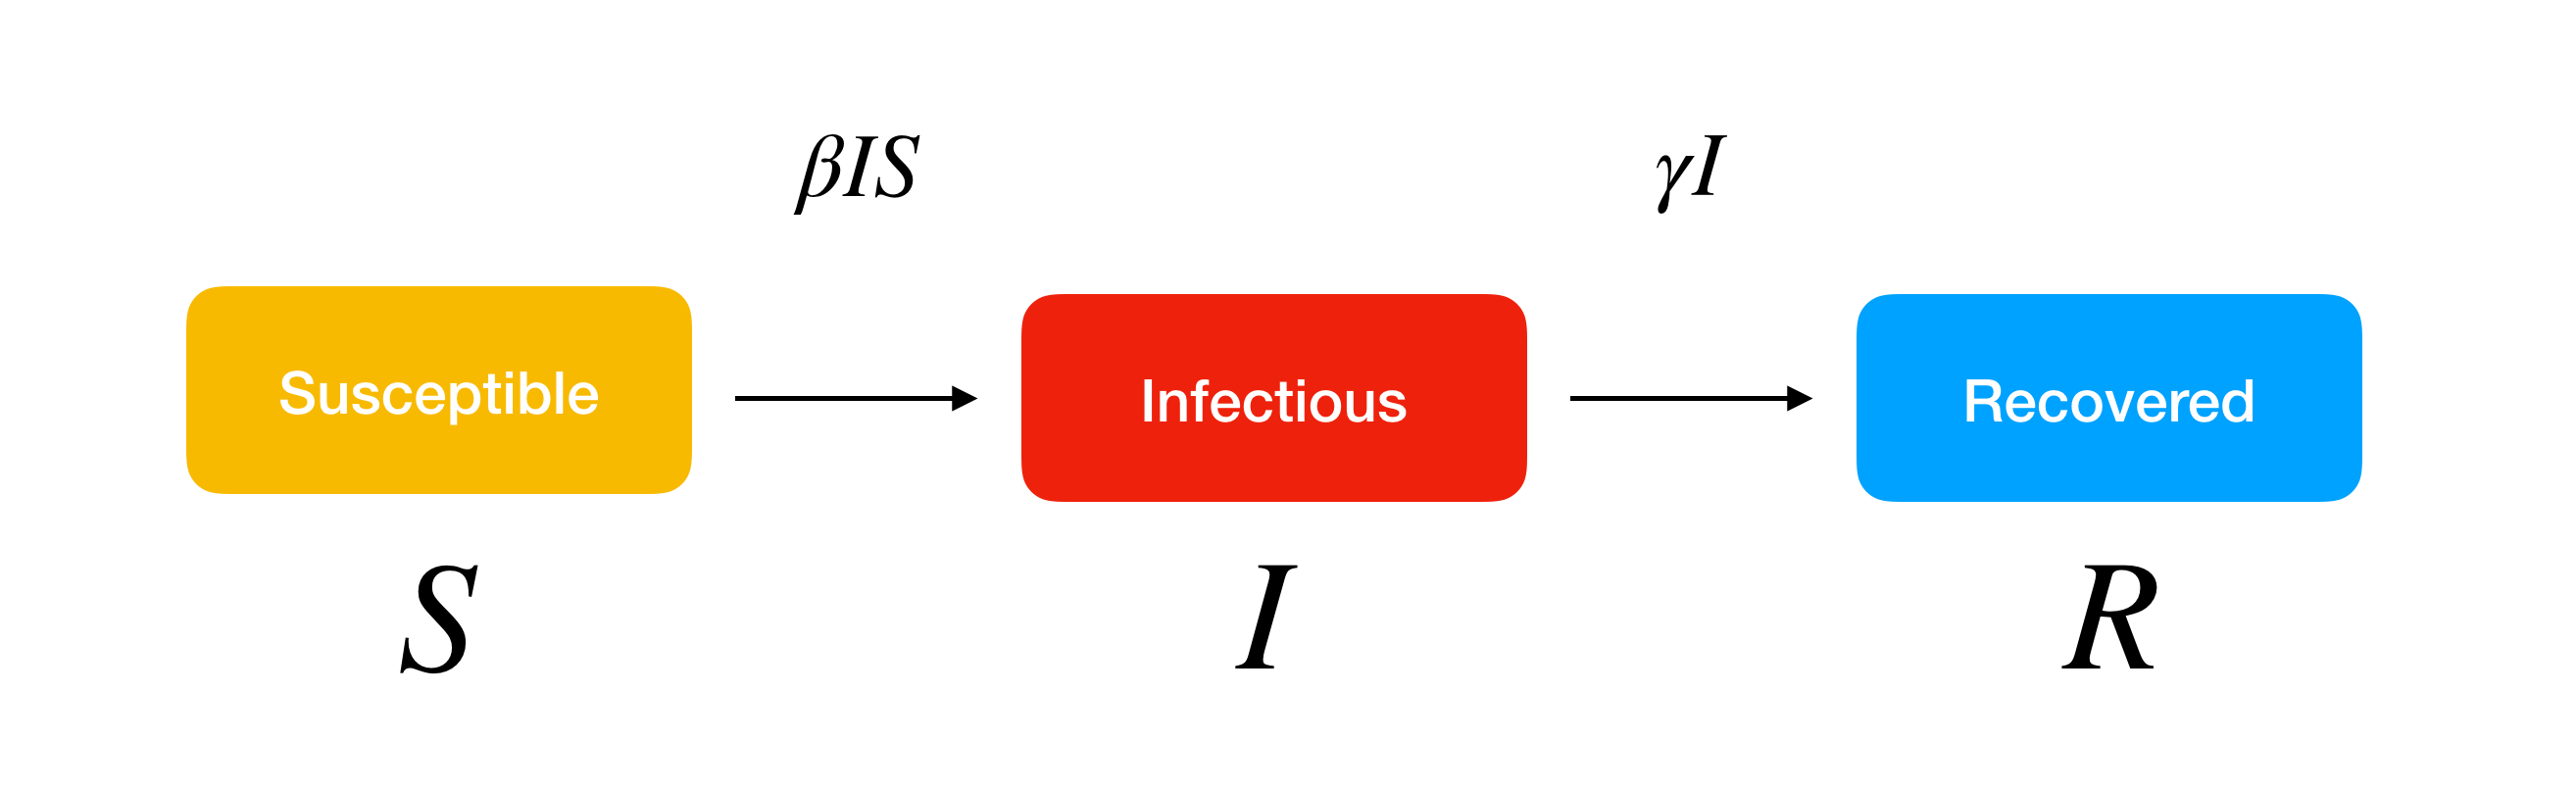
\includegraphics[width=10cm]{images/sir.png}
\centering
\caption{SIR Flow model \cite{sir-model-flow}}
\label{fig:sir-flow}
\end{figure}

\subsubsection{Model parameters}
To understand the SIR model, we need to define a few other parameters.
\begin{itemize}
    \item \textbf{Transmission rate ($\beta $)}: This is the rate at which people are getting infected. In other words, it is the rate at which those in the Susceptible group turn move into the Infected group. This is also called this \textbf{infection rate}.
    \item \textbf{Recovery rate ($\gamma $)}: This is the rate at which people are recovering from the disease. In other words, it is the rate at which those in the Infected group move into the Removed group. The recovery rate depends on how many days the infection lasts. According to the World Health Organization, For COVID-19, 14 days is the maximum number of days for the incubation period. 5 days is the average incubation period \cite{who-website}. Based on the number of days an infected person can spread the disease $\textbf{D}$, we can derive the recovery rate as:
    \begin{equation}
        \label{eq1}
        \gamma = \frac{1}{D}
    \end{equation}
\end{itemize}

Given transmission rate ($\beta$) and $D$, we can derive the basic \textbf{reproduction number $R_{0}$} as:
\begin{equation}
    \label{eq6}
    R_{0} = \beta * D = \frac{\beta}{\gamma}
\end{equation}

$R_{0}$ represents how many healthy people the average infected individual transmits the virus to. If it is high, the probability of pandemic is also higher.

We would also like to note that the values for $\beta$ and $\gamma$ and how they change are very relatable to the measures being taken to fight the pandemic. In particular:
\begin{itemize}
    \item $\beta$ can be thought of as a measure of how quickly the infected individuals spread the virus to susceptible individuals. We may not have any effect on some variables, like the virulence of the disease, but the effectiveness of human behaviors like social distancing and good hygiene will have a direct impact on the value of $\beta$.
    \item Factors that may influence $\gamma$ include things like the availability of a vaccine or other treatments, hospital bed counts, ventilators, and Personal Protective Equipment (PPE) for health care workers.
\end{itemize}

At any given time (t) during the pandemic, we want to know the number of infected, susceptible, recovered, and fatalities. For this, we use ordinary differential equations to describe the rate of change of each group in the SIR model. The SIR model can be expressed by the following set of ordinary differential equations.

\begin{equation}
    \label{eq2}
    \frac{dS}{dt} = - \frac{\beta * I(t) * S(t)}{N}
\end{equation}

\begin{equation}
    \label{eq3}
    \frac{dI}{dt} = \frac{\beta * I(t) * S(t)}{N} - \gamma * I(t) 
\end{equation}

\begin{equation}
    \label{eq4}
    \frac{dR}{dt} = \gamma * I(t) 
\end{equation}

\begin{equation}
    \label{eq5}
    N = S + I + R
\end{equation}

where \textbf{N} is the total population.

\subsubsection{Modeling COVID-19}
As we mentioned in our Solution section, we begin our analysis by starting with a basic SIR model and some historical data that can help us make predictions for the number of individuals in the S, I, and R groups at some point in the future. This gives us an idea of how the virus will spread in the coming months. 

Our mechanism for creating these projections are based on the fact that the SIR model has two parameters ($\beta$, and $\gamma$), and we can use their historical values to anticipate how they will change in the future. Focusing on this method is advantageous for several reasons:
\begin{itemize}
    \item Predicting future values of $S(t)$, $I(t)$, and $R(t)$ is complicated by the fact that these functions have exponential behavior and generally are not easily modeled by common techniques like polynomial regression. In addition, they may seem removed from human intuition as well, because of their same exponential rates of change. On the other hand, given the appropriate machinery, estimating $\beta(t)$ and $\gamma(t)$ may be more realistic because they are not exponential.
    \item Given that $\beta$ and $\gamma$ are the actual model parameters, and have a causal relationship to the $S$, $I$, and $R$ curves, it makes more sense to estimate the model parameters and run the model in the forward direction to make projections, rather than estimating the model output and solving for the parameters in the reverse direction.
    \item As we noted above, there is some human intuition behind these parameters because their values can be linked to real world phenomenon. Therefore, modeling $\beta$ and $\gamma$ accurately would give us a better understanding of how factors like social distancing, contact tracing, and others have a direct relationship with the model, allowing us to separate and analyze each of these causal forces independently.
\end{itemize}

\subsubsection{Historical transmission rate (beta)}
We treat the Transmission rate (beta) as a regression problem. $\beta$ at time t can be represented as a function of time: $\beta(t)$. Therefore our investigation is reduced to a regression problem.  We tried several extrapolation and regression techniques to achieve this goal:
\begin{itemize}
    \item Linear Regression
    \item Quadratic Regression
    \item Weighted Average of $\beta(t)$ values with Exponential Decay
    \item Weighted Average of $\beta'(t)$ values (Slope) with Exponential Decay
    \item Neural Network Regression
\end{itemize}

While the regression methods are self-explanatory, the weighted average techniques are a custom extrapolation technique that we created for this project. In these cases, we work backward through the samples in the sample period, and assign a weight to each sample based on an exponentially decaying memory factor, $\alpha^i, \alpha < 1$. This means that samples closer to the end of the sample time series (and closer to the prediction time frame) will be more influential in the future $\beta(t)$ estimate.

We have implemented two varieties of this summarization technique:
\begin{itemize}
    \item In the first variant, we summarize the \textbf{values} of $\beta(t)$ directly. Obviously, this prevents us from making predictions outside of the historical range of $\beta(t)$, but in many cases, the $\beta(t)$ function tends to be a decreasing function after an initial spike, so, as we will see, it gives reasonable results for countries that are further along in their progression, and are currently in the flattening phase.
    \item The second variant summarizes weighted slope values (which can also be thought of as $\beta'(t)$ values) at a sample. Then, this aggregated slope estimate is combined with the end of the $\beta(t)$ value at the end of the observation period to extrapolate the data and generate a future estimate.
\end{itemize}

Note that we investigated the use of a neural network to predict future values of $\beta(t)$, but decided against using it for three main reasons, listed below:
\begin{enumerate}
    \item The neural network has a large number of parameters, and our data size is not quite large enough to train it sufficiently, so our variance values were very large.
    \item The training time is slow, so evaluating different variations of models is inefficient.
    \item In terms of flexibility, the input size is fixed, so we need to create and train a new network model for every sample size, which is cumbersome.
\end{enumerate}

These methods are all parametric techniques, so we had to experiment with different values for all of these models to see what works best. Figure \ref{fig:historical-transmission-rate-us} shows the historical transmission rate for the United States.

\begin{figure}[h]
    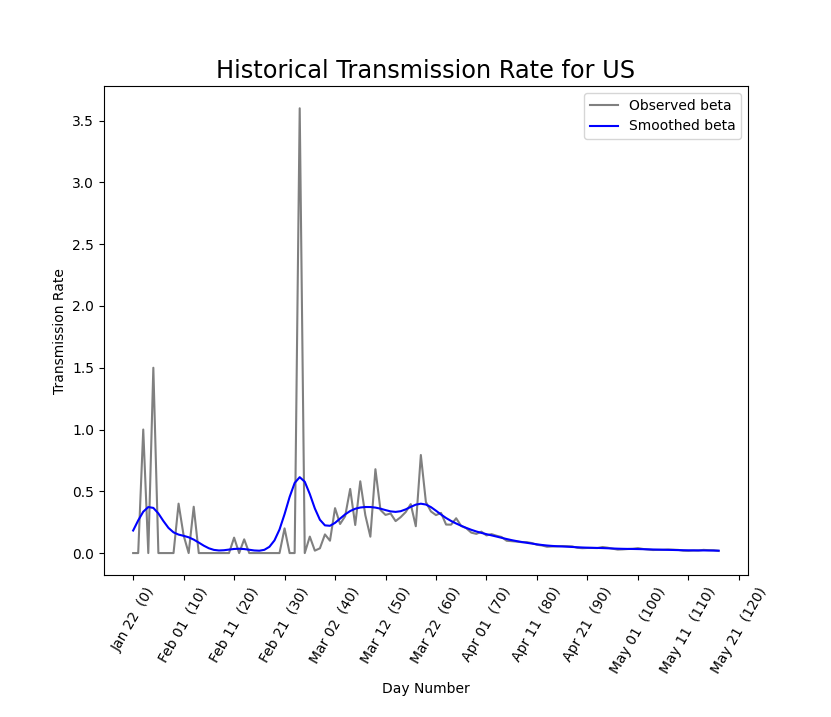
\includegraphics[width=16cm]{images/historical-transmission-rate-US.png}
    \centering
    \caption{Historical transmission rate for US}
    \label{fig:historical-transmission-rate-us}
\end{figure}


\subsubsection{Model Selection}
%copied from the presentation
To determine the best method for estimating future values of $\beta(t)$, we performed the following steps:
\begin{enumerate}
    \item Reserved the last two weeks of the data to run our candidate models against. We refer to all data preceding this time frame as the \textit{learning period}, and the final two weeks as the \textit{prediction period}. We chose a two week prediction period because that duration is consistent with the validation time frames for others in the field of COVID-19 model generation \cite{latest-models}. 
    \item Create as combinations of models using different model types and a range of fixed parameters. We generated  1715 different models from the basic types mentioned in the previous list.
    \item For each of the 188 countries in the data set, run the model to create future values of $\b(t)$, and score the results, using RMSE (root mean square error) values. These values are computed by comparing the projected $I(t)$ values from the model with the actual $I(t)$ values. This equates to approximately 322,000 individual SIR simulations for a 14 day period.
    \item Aggregate the results and normalize RMSE values by country. We do this by simply dividing all RMSE values based on a country's data set by the \textit{minimal} RMSE value for that country. Larger countries with a higher population, or countries further along in the outbreak will have larger raw RMSE values than other countries, so this method gives us \textit{relative errors}, allowing us to compare the various models more directly.
    \item Choose the model that has the best average case performance for all the countries.
    \item Analyze model results along various dimensions and parameter ranges to explore trends and identify potential improvements.
\end{enumerate}

\subsubsection{Model Parameters}
The characteristics of the most important model parameters are described below.
\begin{enumerate}
    \item \textbf{Sample Size}. This value answers the question of how many preceding points we look at while generating the prediction. We always look at the most recent set of points, working our way backward from the end of the learning period. Values for this parameter range between 1 and 60.
    \item \textbf{Memory Factor}. As described earlier, for the value and slope based models, we use an exponential decay function applied to the points to impact how much weight they carry in the prediction. Values for the memory factor range between 0.9 and 1.0. This functions equivalently to an $\alpha$ decay parameter used in many other algorithms.
    \item \textbf{Smoothing Value}. This is a constant, typically represented by $\sigma$ that roughly determines the standard deviation Gaussian filter that we use for smoothing of the observed $\beta(t)$ values. When generating our models, we tried values for this parameter ranging from 1.5 to 4. The behavior of different values in this range is shown below. Note that we are always using these smoothed $\beta(t)$ values for our predictions because the actual $\beta(t)$ values calculated from the historical data are far too volatile to make meaningful predictions.
\end{enumerate}

\begin{figure}[h]
    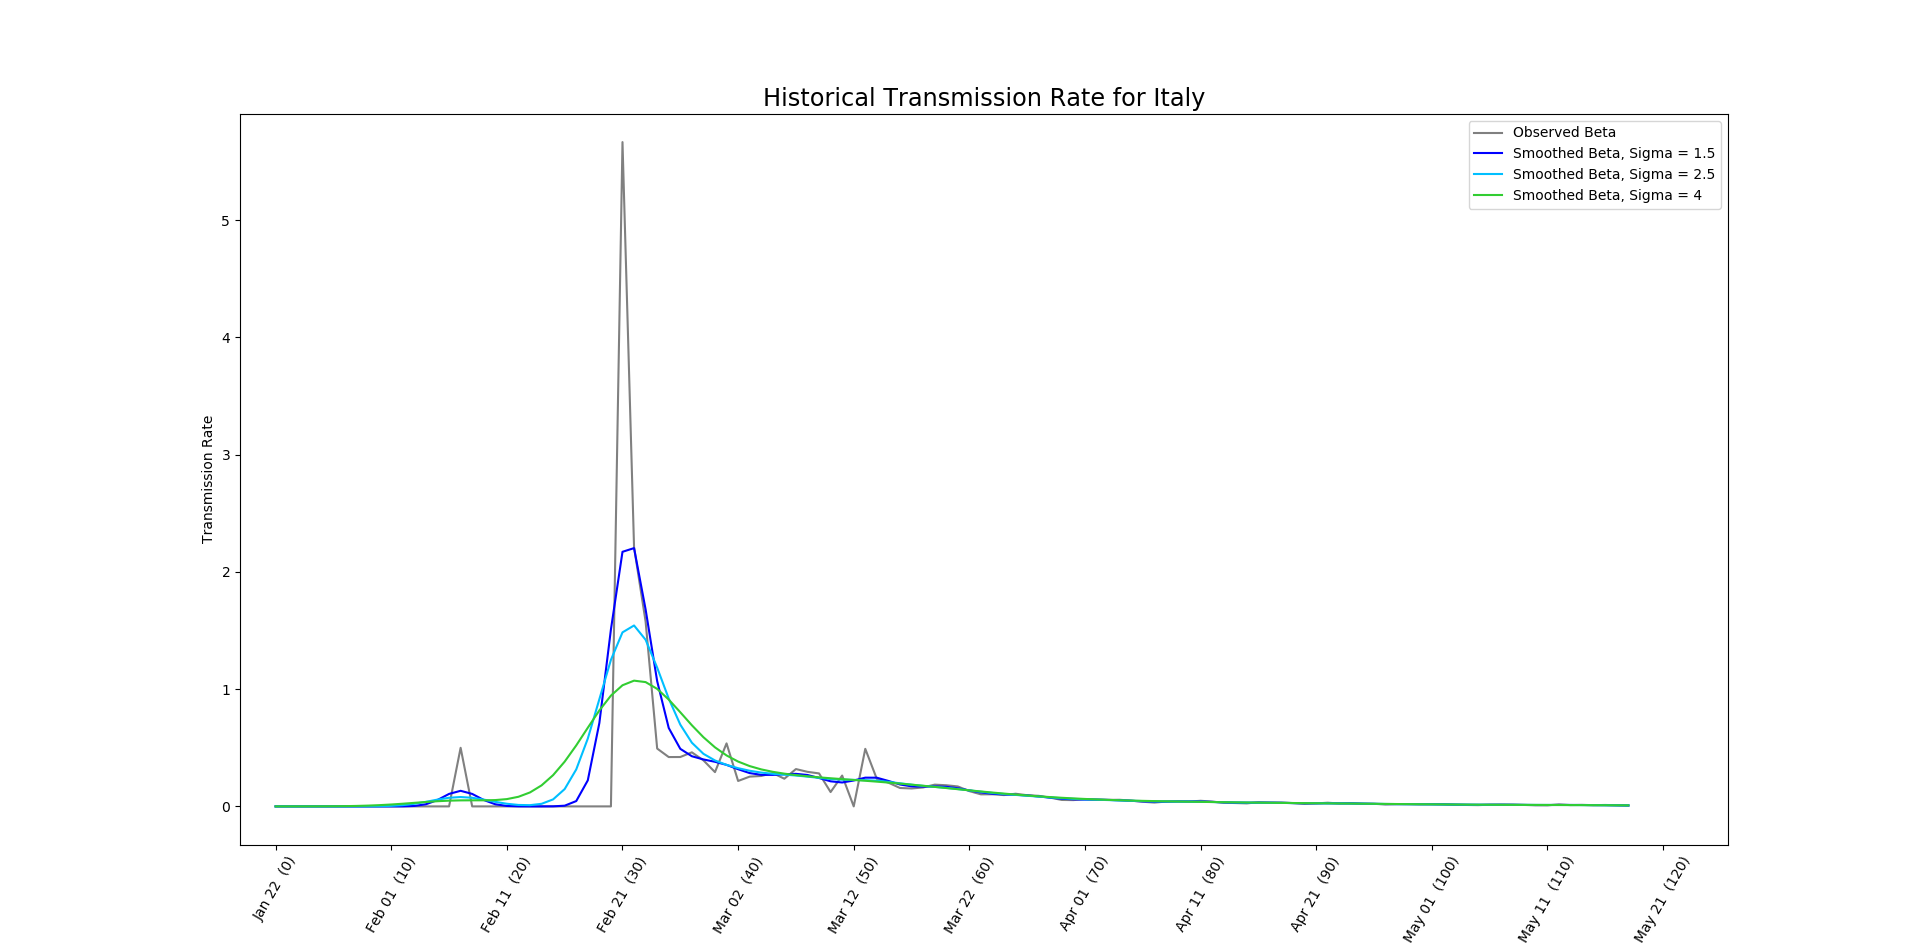
\includegraphics[width=16cm]{images/ItalyTransmission.png}
    \centering
    \caption{Impact of Changing the Smoothing Factor, $\sigma$, on the Historical $\beta(t)$ Values for Italy}
    \label{fig:italy-transmission}
\end{figure}

In addition to these main parameters, we also support 3 different interpolation techniques to fill in $\beta(t)$ predictions based off of a single extrapolation, typically two weeks in the future. The methods we support are below
\begin{itemize}
    \item \textbf{Constant}. Use the estimate of $\beta(t)$for all 14 days in the prediction interval
    \item \textbf{Linear}. Interpolate from the last observed $\beta(t)$value in the learning period to the predicted value after 14 days
    \item \textbf{Quadratic}. Connect the observed $\beta(t)$ curve with a parabola that matches the slope and value of the last observed $\beta$ value at the end of the learning period and is equal to the predicted beta value after 14 days.
\end{itemize}

\section{Experimental results and analysis}
After performing the above experimentation, we were able to closely analyze the performance characteristics of the various candidate models. One of the first things that we computed was to find the best model for each country's data. The relative performance of each model category is shown below.

\begin{figure}[h]
    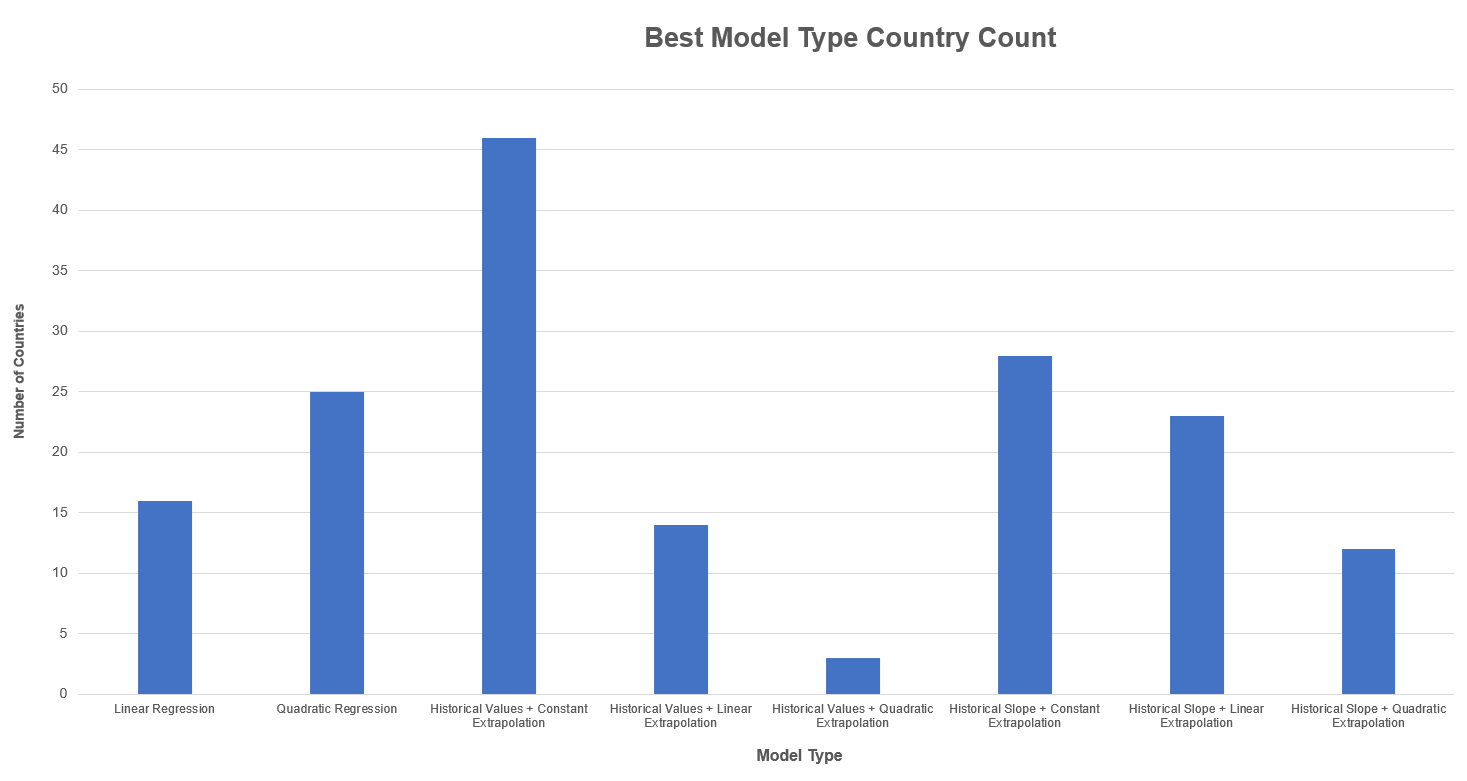
\includegraphics[width=16cm]{images/CountryCount.png}
    \centering
    \caption{Best Models for Each Country, by Category}
    \label{fig:country-count}
\end{figure}

One of the important takeaways from this result is that all model categories are represented, which means that there is not a single model type that strongly outperforms the other candidate models. This fact is an indicator of how difficult the regression problem for $\beta(t)$ is.

We also note that the best model for the United States is a Quadratic Regression model with 10 samples. In general, the countries that fit to quadratic regression or interpolation well are those that are still experiencing large (nonlinear) swings in their numbers. In a qualitative sense, this is an indication that the $\beta(t)$ values United States have not stabilized yet. On the other hand, countries that are modeled by linear or constant models typically are far enough along in the recovery period that their $\beta(t)$ function has flattened out.

We also reviewed the relationship between average model error and the number of sample points, separated by model categories. This output is shown below.

\begin{figure}[h]
    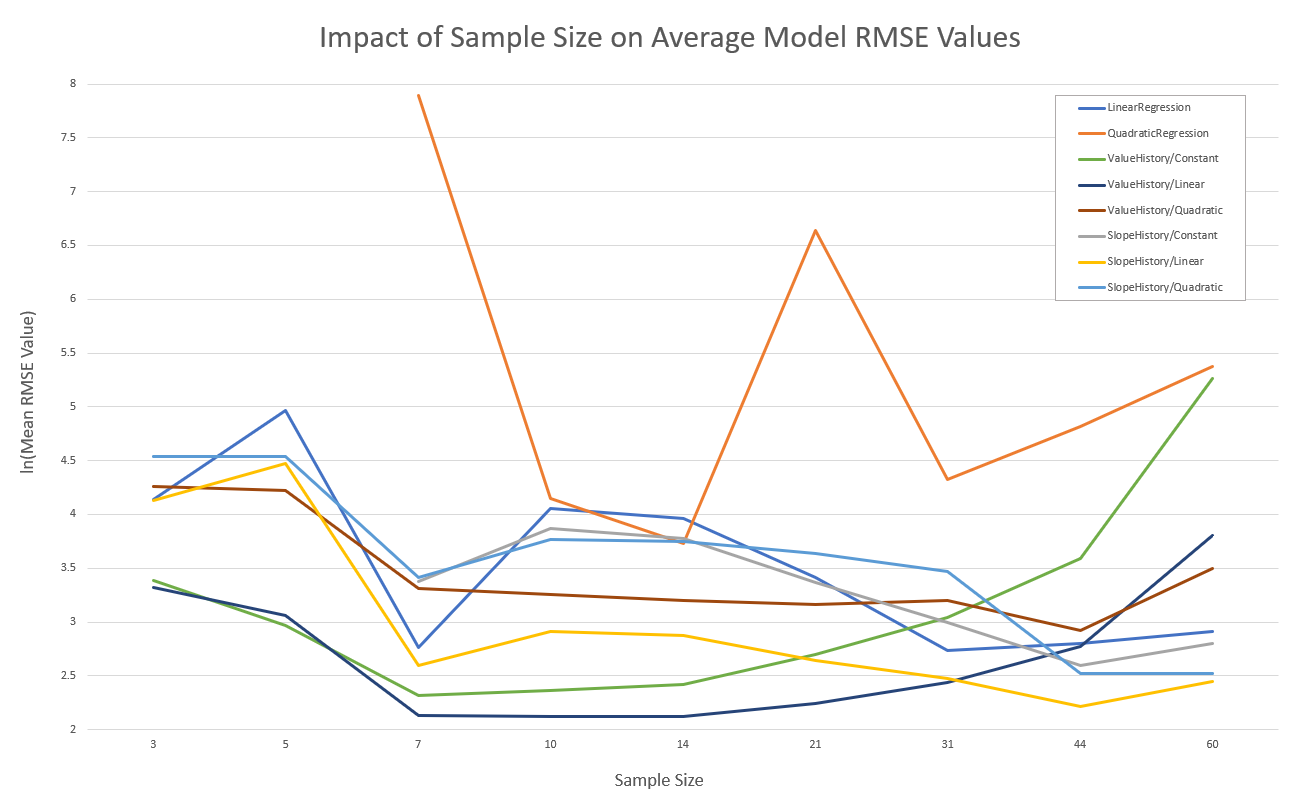
\includegraphics[width=16cm]{images/SampleSizeGraph.png}
    \centering
    \caption{Impact of Sample Size on Model Error}
    \label{fig:sample-size-graph}
\end{figure}

Note that the y-scale is logarithmic. This shows that the quadratic models (orange line) generally have higher error rates, and in fact, the values for the sample size = 3 and sample size = 5 points are removed for the quadratic category because of some extremely bad data that would have stretched the graph too much to be useful. However, the general conclusion is that too few sample points or too many sample points will both have a negative impact on model performance.

Our next experiment was to determine the models that performed the best overall. To do this we run each model variant on the data for all of the countries and scale aggregate the normalized error values. Therefore, the model that performs the best for a single country will have a relative error of 1 for that data set.

After collecting the results we see that the best performing overall model is our custom weighted value model with an exponential decay of $\sigma=0.01$ and a sample size of two weeks. Some other observations about these results are:
\begin{itemize}
    \item The average relative error of the top model was 7.72, which means that there is typically another model that performs 8 times better on a random data set. Therefore, the average model is typically not good compared to the best model for a given data set or country.
    \item The distribution of top models is extremely close. The top-ranking 100 models all had average relative error values of less than 12.
    \item This weighted averaging method with exponential decay tends to work well in a variety of cases. However, in general, different models tend to work better for countries in different phases of the pandemic.
    \item The absolute worst models were the quadratic and slope-based approaches with a small sample size (3-7 previous days), and a small smoothing value of 1.5 or 2. This can lead to an incorrect spike at the end of the learning period, drastically throwing off predictions.
\end{itemize}

Based on these results, we can use the above methods to generate longer-term predictions and graph the model results against actual data. The image below shows a 30-day validation scenario for the United States. The green, red, and blue lines for our estimates are our optimistic, pessimistic, and trending estimate (based on the past 7 days). All of these projections are based on how $\beta$ will change, as compared to the historical data. As expected, the true value for the $I(t)$ curve is between our estimates. This is true for most of the countries we looked at.

\begin{figure}[h]
    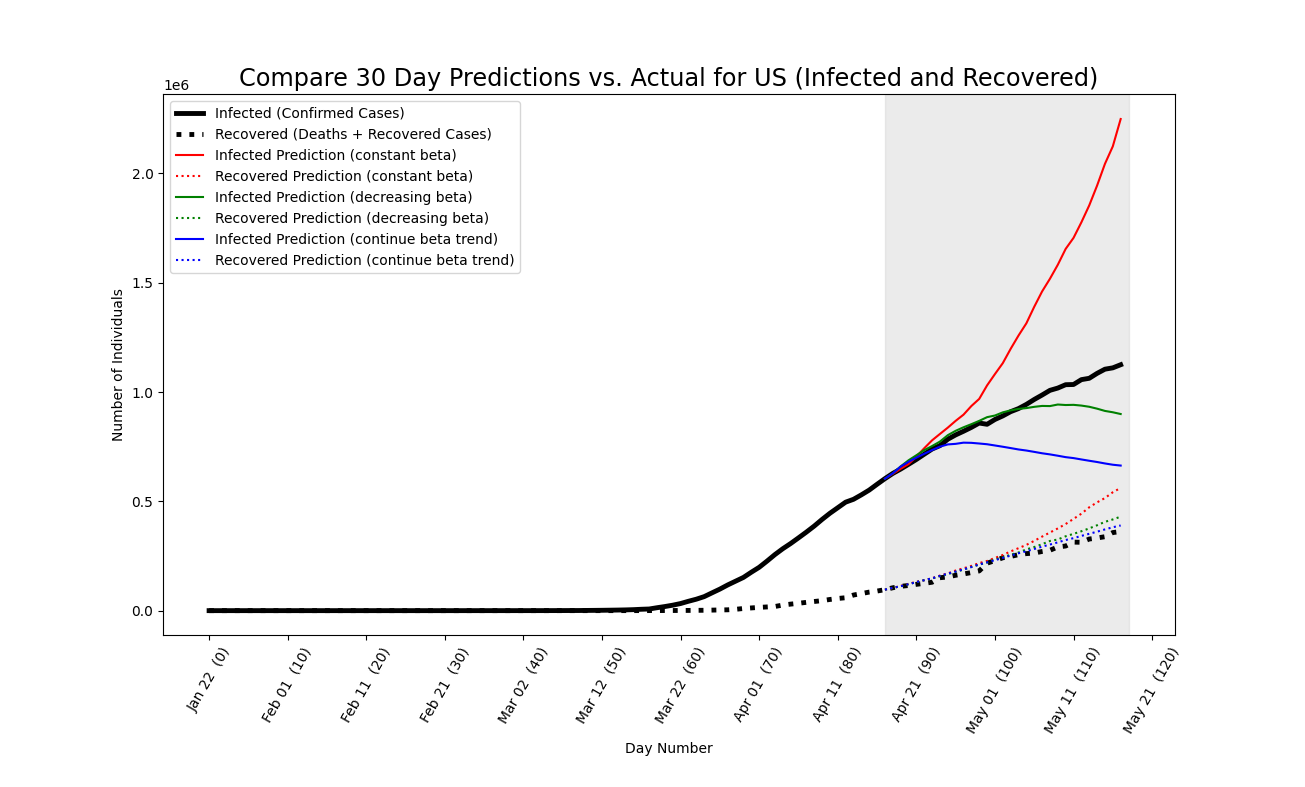
\includegraphics[width=16cm]{images/30-days-prediction-vs-actual-US.png}
    \centering
    \caption{30 Days prediction Vs. Actual values for US}
    \label{fig:30-days-prediction-vs-actual-value}
\end{figure}

In addition, our 60 day scenario for the US data is shown in figure \ref{fig:60-days-prediction-us} below. 

\begin{figure}[h]
    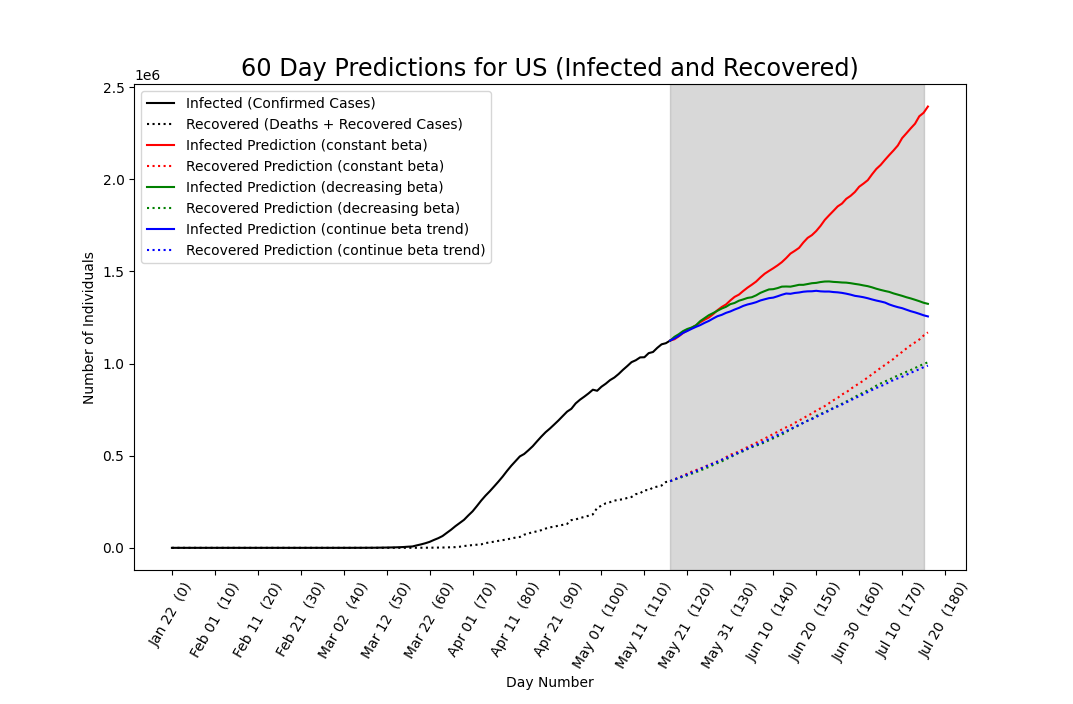
\includegraphics[width=16cm]{images/60-days-prediction-US.png}
    \centering
    \caption{60 Days prediction for US}
    \label{fig:60-days-prediction-us}
\end{figure}

\section{Evaluation}
Given that we are undertaking a regression problem rather than a classification problem, we cannot use traditional metrics based on the confusion matrix generated by the test set.  Rather, we used R2 and mean square error (MSE) scores. We computed these values for each model that we generate. 

In addition to these scores, we also used our models to generate estimates for future counts and then evaluate how close our predictions are once these counts become available. This is a fortunate consequence of analyzing time-series data for an event that is currently in progress.

We ran a ton of different variations of models against the data for all of the countries, does a 14-day prediction, calculate the RMSE score for the prediction, and then aggregates the results from all the models across all of the countries to pick the best one.

\subsubsection{Discussion}
Any model is only as good as the assumptions that we make. Unfortunately, the SIR model makes many overly simplistic assumptions, as a trade-off for simplicity. Many of these assumptions prevent a challenge for us when trying to improve the accuracy of our estimates because the data reflects activities that are happening in reality, but not accounted for in any way by the model.

The sensitivity of the $\beta$ and $\gamma$ parameters and the large impact on the SIR model output, even in cases of exceedingly small discrepancies was also challenging. We found that initial assumptions and the results differ considerably between models. 

Another lesson learned from this project is that the general regression problem is extremely challenging and additional work will be needed to continue to improve the future predictions for the $\beta(t)$ function, as it is generally not a simple function. Our work could probably be extended by adding logic to detect conditions when some models are more applicable than others. 

\section{Conclusion}
We build a curve fitted SIR model to forecast the trajectory of COVID-19 cases for the next 60 days. This model is based on official sources like the WHO and the CDC estimates for case, death, and recovery counts. At the time of writing this paper, the number of cases in the United States is projected to peak around the first week of July with 1.6 million active cases (Confirmed - Recovered - Death). Italy, one of the hardest-hit countries in the European Union will continue its downward trend reach 13000 active cases by the first week of July. Brazil, on the other hand, is on an exponential growth phase and is continuing to rise exponential reaching 2.5 million active cases by the first week of July. This model can be applied to any other country. COVID-19 is still an ongoing pandemic and the spread of this disease largely depends on each country's policies and social distancing measures.


\subsection{Authors and Contributions}
William Austin and Prakash Dhimal jointly investigated the problem, analyzed and interpreted the data, developed the SIR model, implemented regression analysis to project the transmission rate, and evaluated the performance of the models for this paper.

\nocite{epidemic-calculator}
\bibliographystyle{plain}
\bibliography{report}



\pagebreak


\listoffigures

% if you need to show code
% \lstlistoflistings


%end of the document
\end{document}



